\section{微面模型}\label{sec:微面模型}

许多建模表面反射和透射的基于几何光学的方法
都基于一个观点即粗糙表面可以建模为
小的\keyindex{微面}{microfacet}{}合集。
由微面构成的曲面经常建模为高度场\sidenote{译者注:原文heightfield。},
其中微面的朝向分布是作统计上的描述。
\reffig{8.12}展示了相对粗糙表面的横截面和光滑得多的微面表面。
当区别不明显时,我们将用术语\keyindex{微曲面}{microsurface}{}来
描述微面曲面,用\keyindex{宏曲面}{macrosurface}{}来描述基本的光滑曲面
(即由\refvar{Shape}{}表示的)。
\begin{figure}[htbp]
    \centering
    \includegraphics[width=0.75\linewidth]{Pictures/chap08/Roughsmoothmicrofacets.eps}
    \caption{微面曲面模型经常由给出微面法线${\bm n}_{\mathrm{f}}$关于
        曲面法线$\bm n$的分布的函数来描述。(a)微面法线变化越大,表面越粗糙。
        (b)光滑表面的微面法线变化相对较小。}
    \label{fig:8.12}
\end{figure}

基于微面的BRDF模型通过统计上对来自大量微面的光的散射建模来奏效。
如果我们假设被照明的微分区域$\mathrm{d}A$比起单个微面的尺寸相对大些,
则有大量微面被照亮且它们合起来的表现决定了观察到的散射。

微面模型的两个主要构成是\keyindex{刻面}{facet}{}
\sidenote{译者注:暂未查到facet在图形学中的专门翻译。}分布的表示
和描述光如何从单个微面散射的BRDF。有了这些,
任务是推导BRDF的解析表达式以描述来自这类曲面的散射。
尽管镜面透射对于建模许多透明材料很有用,
但对于微面BRDF,完美镜面反射是最常用的,
(下节介绍的)Oren-Nayar模型把微面看作朗伯反射体。

为了计算来自这类模型的反射,需要考虑微面级的局部光效应(\reffig{8.13})。
微面可能被另一刻面遮挡,可能处在相邻微面的阴影下,
或者\keyindex{互反射}{interreflection}{}可能
造成微面反射出比直接照明量和低层级微面BRDF预计的还多的光。
基于微面的特定BRDF模型以各种精确程度考虑了这些效应的每一种。
一般方法是做出尽可能最好的近似,且仍得到计算简单的表达式。
\begin{figure}[htbp]
    \centering
    \includegraphics[width=\linewidth]{Pictures/chap08/Maskingshadowinginterreflection.eps}
    \caption{微面反射模型要考虑的三种重要几何效应。(a)遮掩(masking):
        考虑的微面因为另一微面的遮挡而对观察者不可见。(b)阴影(shadowing):
        类似地,光无法到达微面。(3)互反射:光在到达
        观察者之前于微面之间反弹。}
    \label{fig:8.13}
\end{figure}

\subsection{Oren-Nayar漫反射}\label{sub:Oren-Nayar漫反射}
\citet{10.1145/192161.192213}观察到真实世界物体不会展现完美朗伯反射。
具体地,当照明方向接近观察方向时,粗糙曲面通常显得更亮。
他们用含有单个参数$\sigma$即微面朝向角度标准差的球面高斯分布
描述的V形微面\sidenote{译者注:也称“V形槽微面”。}构建了描述粗糙曲面的反射模型。

在V形假设下,可以通过只考虑相邻微面来处理互反射;
\citeauthor{10.1145/192161.192213}利用这点
推导出对凹槽\sidenote{译者注:原文groove。}集的整体反射建模的BRDF。

所得模型考虑了微面间的阴影、遮掩和互反射,但没有解析解,
所以他们发现下列近似拟合得很好
\sidenote{译者注:原文可能因笔误写作$f_{\mathrm{r}}({\bm\omega}_{\mathrm{i}},{\bm\omega}_{\mathrm{o}})$,
    与前后文记号不一致,这里笔者改回为$f_{\mathrm{r}}({\bm\omega}_{\mathrm{o}},{\bm\omega}_{\mathrm{i}})$.}:
\begin{align*}
    f_{\mathrm{r}}({\bm\omega}_{\mathrm{o}},{\bm\omega}_{\mathrm{i}})=\frac{R}{\pi}(A+B\max(0,\cos(\varphi_{\mathrm{i}}-\varphi_{\mathrm{o}}))\sin\alpha\tan\beta)\, ,
\end{align*}
其中如果$\sigma$单位是弧度,则
\begin{align*}
    A      & =1-\frac{\sigma^2}{2(\sigma^2+0.33)}\, ,           \\
    B      & =\frac{0.45\sigma^2}{\sigma^2+0.09}\, ,            \\
    \alpha & =\max(\theta_{\mathrm{i}},\theta_{\mathrm{o}})\, , \\
    \beta  & =\min(\theta_{\mathrm{i}},\theta_{\mathrm{o}})\, .
\end{align*}

\begin{figure}[htbp]
    \centering
    \subfloat[朗伯]{\includegraphics[width=0.7\linewidth]{Pictures/chap08/f8-14a.png}\label{fig:8.14.1}}\\
    \subfloat[Oren-Nayar]{\includegraphics[width=0.7\linewidth]{Pictures/chap08/f8-14b.png}\label{fig:8.14.2}}
    \caption{(a)来自\refvar{LambertianReflection}{}模型的标准漫反射和
        (b)$\sigma$参数为20度的\refvar{OrenNayar}{}模型渲染的龙模型。
        注意用Oren-Nayar模型时暗色轮廓边缘反射增加了,浅色明暗边缘通常也更干脆
        (感谢Christian Schüller提供的模型)。}
    \label{fig:8.14}
\end{figure}

这里的实现在构造函数中预先计算和保存参数$A$与$B$的值
以节约稍后计算BRDF的工作量。\reffig{8.14}比较了理想漫反射和Oren-Nayar模型渲染的区别。
\begin{lstlisting}
`\initcode{OrenNayar Public Methods}{=}`
`\initvar{OrenNayar}{}`(const `\refvar{Spectrum}{}` &R, `\refvar{Float}{}` sigma) 
    : `\refvar{BxDF}{}`(`\refvar{BxDFType}{}`(`\refvar[BSDFREFLECTION]{BSDF\_REFLECTION}{}` | `\refvar[BSDFDIFFUSE]{BSDF\_DIFFUSE}{}`)), `\refvar[OrenNayar::R]{R}{}`(R) {
    sigma = `\refvar{Radians}{}`(sigma);
    `\refvar{Float}{}` sigma2 = sigma * sigma;
    `\refvar[OrenNayar::A]{A}{}` = 1.f - (sigma2 / (2.f * (sigma2 + 0.33f)));
    `\refvar[OrenNayar::B]{B}{}` = 0.45f * sigma2 / (sigma2 + 0.09f);
}
\end{lstlisting}
\begin{lstlisting}
`\initcode{OrenNayar Private Data}{=}`
const `\refvar{Spectrum}{}` `\initvar[OrenNayar::R]{R}{}`;
`\refvar{Float}{}` `\initvar[OrenNayar::A]{A}{}`, `\initvar[OrenNayar::B]{B}{}`;
\end{lstlisting}

比起直接变换基本方程,三角恒等式的应用可以极大提升求值例程的效率。
实现从计算$\sin\theta_{\mathrm{i}}$和$\sin\theta_{\mathrm{o}}$的值开始。
\begin{lstlisting}
`\refcode{BxDF Method Definitions}{+=}\lastnext{BxDFMethodDefinitions}`
`\refvar{Spectrum}{}` `\refvar{OrenNayar}{}`::`\initvar[OrenNayar::f]{f}{}`(const `\refvar{Vector3f}{}` &wo, const `\refvar{Vector3f}{}` &wi) const {
    `\refvar{Float}{}` sinThetaI = `\refvar{SinTheta}{}`(wi);
    `\refvar{Float}{}` sinThetaO = `\refvar{SinTheta}{}`(wo);
    `\refcode{Compute cosine term of Oren-Nayar model}{}`
    `\refcode{Compute sine and tangent terms of Oren-Nayar model}{}`
    return `\refvar[OrenNayar::R]{R}{}` * `\refvar{InvPi}{}` * (`\refvar[OrenNayar::A]{A}{}` + `\refvar[OrenNayar::B]{B}{}` * maxCos * sinAlpha * tanBeta);
}
\end{lstlisting}

为了计算项$\max(0,\cos(\varphi_{\mathrm{i}}-\varphi_{\mathrm{o}}))$,
我们可以应用三角恒等式
\begin{align*}
    \cos(a-b)=\cos a\cos b+\sin a\sin b\, ,
\end{align*}
这样我们只需要计算$\varphi_{\mathrm{i}}$和$\varphi_{\mathrm{o}}$的正弦和余弦。
\begin{lstlisting}
`\initcode{Compute cosine term of Oren-Nayar model}{=}`
`\refvar{Float}{}` maxCos = 0;
if (sinThetaI > 1e-4 && sinThetaO > 1e-4) {
    `\refvar{Float}{}` sinPhiI = `\refvar{SinPhi}{}`(wi), cosPhiI = `\refvar{CosPhi}{}`(wi);
    `\refvar{Float}{}` sinPhiO = `\refvar{SinPhi}{}`(wo), cosPhiO = `\refvar{CosPhi}{}`(wo);
    `\refvar{Float}{}` dCos = cosPhiI * cosPhiO + sinPhiI * sinPhiO;
    maxCos = std::max((`\refvar{Float}{}`)0, dCos);
}
\end{lstlisting}

最后,求得项$\sin\alpha$和$\tan\beta$.
注意无论${\bm\omega}_{\mathrm{i}}$或${\bm\omega}_{\mathrm{o}}$中的哪一个,
有更大的$\cos\theta$(即更大的$z$分量)就有更小的$\theta$.
我们可以用该方法开头计算的近似正弦值来设定$\sin\alpha$.
然后用恒等式$\displaystyle\tan\theta=\frac{\sin\theta}{\cos\theta}$计算正切。
\begin{lstlisting}
`\initcode{Compute sine and tangent terms of Oren-Nayar model}{=}`
`\refvar{Float}{}` sinAlpha, tanBeta;
if (`\refvar{AbsCosTheta}{}`(wi) > `\refvar{AbsCosTheta}{}`(wo)) {
    sinAlpha = sinThetaO;
    tanBeta = sinThetaI / `\refvar{AbsCosTheta}{}`(wi);
} else {
    sinAlpha = sinThetaI;
    tanBeta = sinThetaO / `\refvar{AbsCosTheta}{}`(wo);
}
\end{lstlisting}

\subsection{微面分布函数}\label{sub:微面分布函数}
反射模型所基于的微面展现出完美镜面反射和透射时,
其对来自各种光泽材料的光散射的建模已经很高效了,包括金属、塑料和磨砂玻璃。
在我们讨论这些模型的辐射度量细节前,
我们将首先介绍概括了其几何属性的抽象。
这里的代码包括了两个广泛使用的微面模型的实现。
这些代码都在文件\href{https://github.com/mmp/pbrt-v3/tree/master/src/core/microfacet.h}{\ttfamily core/microfacet.h}
和\href{https://github.com/mmp/pbrt-v3/tree/master/src/core/microfacet.cpp}{\ttfamily core/microfacet.cpp}中。

\refvar{MicrofacetDistribution}{}定义了
由微面实现提供的接口及其常用功能。
\begin{lstlisting}
`\initcode{MicrofacetDistribution Declarations}{=}\initnext{MicrofacetDistributionDeclarations}`
class `\initvar{MicrofacetDistribution}{}` {
public:
    `\refcode{MicrofacetDistribution Public Methods}{}`
protected:
    `\refcode{MicrofacetDistribution Protected Methods}{}`
    `\refcode{MicrofacetDistribution Protected Data}{}`
};
\end{lstlisting}

微面曲面的一个重要特性由分布函数$D({\bm\omega}_{\mathrm{h}})$表示,
它给出了曲面法线为${\bm\omega}_{\mathrm{h}}$的微面的微分面积
(回想\reffig{8.12}展示了曲面的粗糙度是怎样和微面法线分布函数相联系的)。
在pbrt中,微面分布函数和\refvar{BxDF}{}在相同的BSDF坐标系下定义;
这样,完全光滑的曲面可由仅当${\bm\omega}_{\mathrm{h}}$等于
曲面法线时才取非零值的$\delta$分布描述:$D({\bm\omega}_{\mathrm{h}})=\delta({\bm\omega}_{\mathrm{h}}-(0,0,1))$.

微面分布函数必须规范化以保证它们的物理合理性
\sidenote{译者注:除了下文的归一化约束,$D({\bm\omega}_{\mathrm{h}})$还有非负性。}。
直观上,如果我们考虑微曲面上沿法线方向$\bm n$的入射光线,
则每条光线一定和微面曲面恰好相交一次。更形式化地,
给定微曲面的微分面积$\mathrm{d}A$,则该区域之上微面的投影面积
一定等于$\mathrm{d}A$(\reffig{8.15})
\sidenote{译者注:该公式积分区域取半空间并不严谨,实际上应取全空间才对,否则会漏掉背面朝向的微面面积。
    有关$D({\bm\omega}_{\mathrm{h}})$的详细说明可参见笔者编写的\refsec{译者补充:微面模型相关推导}。}。
数学上,这对应着以下条件
\footnote{规范化微面分布的常见错误是在整个立体角上
    而不是投影立体角上执行该积分(即略去的项$\cos\theta_{\mathrm{h}}$),
    这无法保证具有正确分布的高度场存在。}:
\begin{align*}
    \int\limits_{H^2({\bm n})}D({\bm\omega}_{\mathrm{h}})\cos\theta_{\mathrm{h}}\mathrm{d}{\bm\omega}_{\mathrm{h}}=1\, .
\end{align*}
\begin{figure}[htbp]
    \centering
    \includegraphics[width=0.5\linewidth]{Pictures/chap08/MicrofacetnormalizedA.eps}
    \caption{给定曲面上的微分面积$\mathrm{d}A$,
        则微面法线分布函数$D({\bm\omega}_{\mathrm{h}})$必须规范化使得
        该区域上的微面的投影曲面面积等于$\mathrm{d}A$.}
    \label{fig:8.15}
\end{figure}

方法\refvar{MicrofacetDistribution::D}{()}对应函数$D({\bm\omega}_{\mathrm{h}})$;
实现返回具有给定法线向量$\omega$朝向的微面的微分面积。
\begin{lstlisting}
`\initcode{MicrofacetDistribution Public Methods}{=}\initnext{MicrofacetDistributionPublicMethods}`
virtual `\refvar{Float}{}` `\initvar[MicrofacetDistribution::D]{D}{}`(const `\refvar{Vector3f}{}` &wh) const = 0;
\end{lstlisting}

\citet{1987BeckmannSpizzichino}\sidenote{译者注:
    笔者只查到了1987年同名同作者书籍,原文引用为1963年。}提出了
一种广泛使用的基于微面斜率高斯分布的微面分布函数;
我们的实现在类\refvar{BeckmannDistribution}{}中。
\begin{lstlisting}
`\refcode{MicrofacetDistribution Declarations}{+=}\lastnext{MicrofacetDistributionDeclarations}`
class `\initvar{BeckmannDistribution}{}` : public `\refvar{MicrofacetDistribution}{}` {
public:
    `\refcode{BeckmannDistribution Public Methods}{}`
private:
    `\refcode{BeckmannDistribution Private Methods}{}`
    `\refcode{BeckmannDistribution Private Data}{}`
};
\end{lstlisting}

Beckmann-Spizzichino模型的传统定义是
\begin{align}\label{eq:8.9}
    D({\bm\omega}_{\mathrm{h}})=\frac{\mathrm{e}^{-\frac{\tan^2\theta_{\mathrm{h}}}{\alpha^2}}}{\pi\alpha^2\cos^4\theta_{\mathrm{h}}}\, ,
\end{align}
其中如果$\sigma$是微面斜率的均方根\sidenote{译者注:原文RMS。},则$\alpha=\sqrt{2}\sigma$.

定义各向异性分布很有用,即法线分布也随${\bm\omega}_{\mathrm{h}}$的
方位朝向变化。例如,所朝方向垂直于$x$轴的微面对应记为$\alpha_x$,
而$y$轴的为$\alpha_y$,则中间朝向的$\alpha$值可用通过这些值构造的椭圆来插值。

对应的各向异性微面分布函数为
\sidenote{译者注:\refsec{译者补充:微面模型相关推导},
    给出了本节微面分布模型满足规范性的证明。}
\begin{align}\label{eq:8.10}
    D({\bm\omega}_{\mathrm{h}})=\frac{\mathrm{e}^{-\left(\frac{\cos^2\varphi_{\mathrm{h}}}{\alpha_x^2}+\frac{\sin^2\varphi_{\mathrm{h}}}{\alpha_y^2}\right)\tan^2\theta_{\mathrm{h}}}}{\pi\alpha_x\alpha_y\cos^4\theta_{\mathrm{h}}}\, .
\end{align}
注意当$\alpha_x=\alpha_y$时Beckmann-Spizzichino模型
变为原始的各向同性版本。

成员变量\refvar[BeckmannDistribution::alphax]{alphax}{}和
\refvar[BeckmannDistribution::alphay]{alphay}{}都在
\refvar{BeckmannDistribution}{}的构造函数中设定,
它很简单所以这里不再介绍。
\begin{lstlisting}
`\initcode{BeckmannDistribution Private Data}{=}`
const `\refvar{Float}{}` `\initvar[BeckmannDistribution::alphax]{alphax}{}`, `\initvar[BeckmannDistribution::alphay]{alphay}{}`;
\end{lstlisting}

方法\refvar{BeckmannDistribution::D}{()}直接翻译了\refeq{8.10}。
仅有的额外实现细节是必须特殊处理$\tan^2\theta$的无限值。
该情况实际上是有效的——它在完全扫掠的方向上发生。
该情况下,下面的代码最终企图计算$\displaystyle\frac{0}{0}$,
这会得到“not a number”(NaN)值,最终导致为当前像素样本的辐射亮度返回NaN值。
因此,为该情况明确地返回零,也即当$\tan^2\theta_{\mathrm{h}}$趋向
无穷大时$D({\bm\omega}_{\mathrm{h}})$收敛的值。
\begin{lstlisting}
`\initcode{MicrofacetDistribution Method Definitions}{=}\initnext{MicrofacetDistributionMethodDefinitions}`
`\refvar{Float}{}` `\refvar{BeckmannDistribution}{}`::`\initvar[BeckmannDistribution::D]{D}{}`(const `\refvar{Vector3f}{}` &wh) const {
    `\refvar{Float}{}` tan2Theta = `\refvar{Tan2Theta}{}`(wh);
    if (std::isinf(tan2Theta)) return 0.;
    `\refvar{Float}{}` cos4Theta = `\refvar{Cos2Theta}{}`(wh) * `\refvar{Cos2Theta}{}`(wh);
    return std::exp(-tan2Theta * (`\refvar{Cos2Phi}{}`(wh) / (`\refvar[BeckmannDistribution::alphax]{alphax}{}` * `\refvar[BeckmannDistribution::alphax]{alphax}{}`) +
                                  `\refvar{Sin2Phi}{}`(wh) / (`\refvar[BeckmannDistribution::alphay]{alphay}{}` * `\refvar[BeckmannDistribution::alphay]{alphay}{}`))) /
        (`\refvar{Pi}{}` * `\refvar[BeckmannDistribution::alphax]{alphax}{}` * `\refvar[BeckmannDistribution::alphay]{alphay}{}` * cos4Theta);
}
\end{lstlisting}

\citet{Trowbridge:75}提出了另一个有用的微面分布函数
\footnote{该模型也由\citet{10.5555/2383847.2383874}独立推导出,称作“GGX”。}。
其各向异性变体由下式给出:
\begin{align}\label{eq:8.11}
    D({\bm\omega}_{\mathrm{h}})=\frac{1}{\pi\alpha_x\alpha_y\left(1+\left(\frac{\cos^2\varphi_{\mathrm{h}}}{\alpha_x^2}+\frac{\sin^2\varphi_{\mathrm{h}}}{\alpha_y^2}\right)\tan^2\theta_{\mathrm{h}}\right)^2\cos^4\theta_{\mathrm{h}}}\, .
\end{align}

相比于Beckmann-Spizzichino模型,Trowbridge-Reitz模型有更高的拖尾——
在远离曲面法线的方向上它会更慢地降到零。该特性与许多真实世界表面的性质吻合得很好。
见\reffig{8.16}中这两个微面分布函数的图示。
\begin{figure}[htbp]
    \centering
    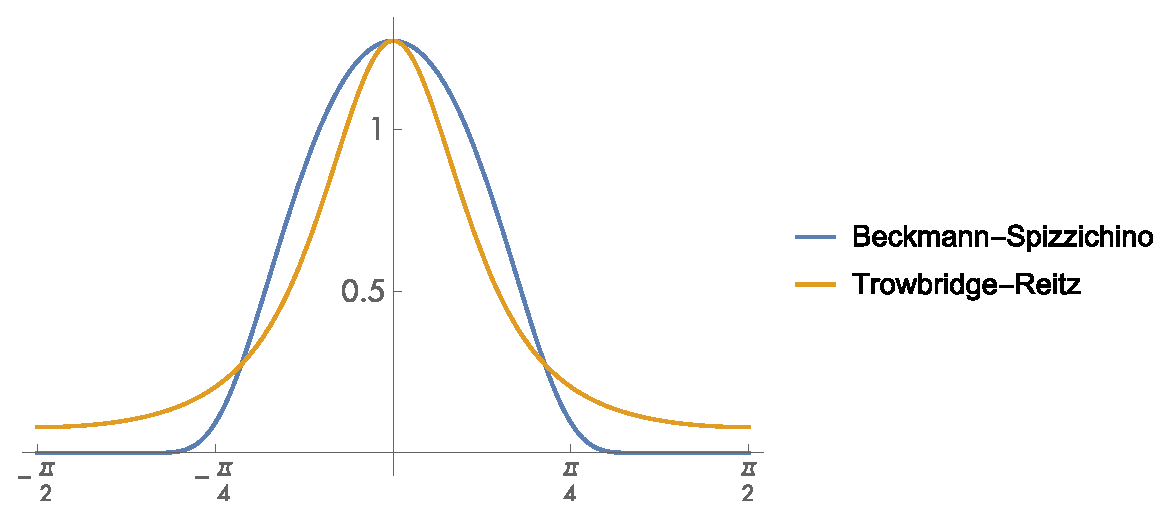
\includegraphics[width=0.75\linewidth]{Pictures/chap08/beckmann-vs-tr-tails.eps}
    \caption{当$\alpha=0.5$时各向同性的Beckmann-Spizzichino和Trowbridge-Reitz微面分布函数
        关于$\theta$的函数图像。注意Trowbridge-Reitz对于更大量级的$\theta$有更高的尾部。}
    \label{fig:8.16}
\end{figure}

\begin{lstlisting}
`\refcode{MicrofacetDistribution Declarations}{+=}\lastnext{MicrofacetDistributionDeclarations}`
class `\initvar{TrowbridgeReitzDistribution}{}` : public `\refvar{MicrofacetDistribution}{}` {
public:
    `\refcode{TrowbridgeReitzDistribution Public Methods}{}`
private:
    `\refcode{TrowbridgeReitzDistribution Private Methods}{}`
    `\refcode{TrowbridgeReitzDistribution Private Data}{}`
};
\end{lstlisting}

比起直接指定$\alpha$的值,用一个$[0,1]$中的标量参数来
指定BRDF的粗糙度会很方便,其中接近零的值对应几乎完美的镜面反射。
这里略去的方法\refvar{RoughnessToAlpha}{()}执行从该粗糙度值到$\alpha$值的映射。
\begin{lstlisting}
`\initcode{TrowbridgeReitzDistribution Public Methods}{=}`
static inline `\refvar{Float}{}` `\initvar{RoughnessToAlpha}{}`(`\refvar{Float}{}` roughness);
\end{lstlisting}
\begin{lstlisting}
`\initcode{TrowbridgeReitzDistribution Private Data}{=}`
const `\refvar{Float}{}` `\initvar[TrowbridgeReitzDistribution::alphax]{alphax}{}`, `\initvar[TrowbridgeReitzDistribution::alphay]{alphay}{}`;
\end{lstlisting}

方法\refvar[TrowbridgeReitzDistribution::D]{D}{()}是直接照着\refeq{8.11}写的。
\begin{lstlisting}
`\refcode{MicrofacetDistribution Method Definitions}{+=}\lastnext{MicrofacetDistributionMethodDefinitions}`
`\refvar{Float}{}` `\refvar{TrowbridgeReitzDistribution}{}`::`\initvar[TrowbridgeReitzDistribution::D]{D}{}`(const `\refvar{Vector3f}{}` &wh) const {
    `\refvar{Float}{}` tan2Theta = `\refvar{Tan2Theta}{}`(wh);
    if (std::isinf(tan2Theta)) return 0.;
    const `\refvar{Float}{}` cos4Theta = `\refvar{Cos2Theta}{}`(wh) * `\refvar{Cos2Theta}{}`(wh);
    `\refvar{Float}{}` e = (`\refvar{Cos2Phi}{}`(wh) / (`\refvar[TrowbridgeReitzDistribution::alphax]{alphax}{}` * `\refvar[TrowbridgeReitzDistribution::alphax]{alphax}{}`) +
               `\refvar{Sin2Phi}{}`(wh) / (`\refvar[TrowbridgeReitzDistribution::alphay]{alphay}{}` * `\refvar[TrowbridgeReitzDistribution::alphay]{alphay}{}`)) * tan2Theta;
    return 1 / (`\refvar{Pi}{}` * `\refvar[TrowbridgeReitzDistribution::alphax]{alphax}{}` * `\refvar[TrowbridgeReitzDistribution::alphay]{alphay}{}` * cos4Theta * (1 + e) * (1 + e));
}
\end{lstlisting}

\subsection{掩模和遮挡}\label{sub:掩模和遮挡}
对于渲染,只有微面法线分布不足以完全表征微曲面。
同样很重要的是,要考虑到一些微面从某给定视角或光照方向看去
会因为它们是背面朝向而不可见(因而其他微面在它们的前方),
以及一些正面朝向的微面区域会因为受到背面朝向微面的遮挡而被隐藏
\sidenote{译者注:在英语中,“mask”和“shadow”都能表示遮盖遮挡之意。
    为了区分这里所述的因观察角度与微面方向相背而引发的遮挡和
    因微面本身粗糙而引发的局部遮挡,英语术语特地选用了这两个意思相同但读写不同的称呼。
    但是在中文里这种做法就显得不太合适,以“遮挡”“遮盖”“遮蔽”之类的近义词作区分
    并不能帮助读者意识到它们的差别,反而更容易引起混淆。
    权衡之下,笔者选用“mask”的另一种翻译——“掩模”(也可作“掩膜”)来增强和“遮挡”的区别感。
    因为该词在图像处理中常常指规定取用哪些像素的布尔量集合,与本文中“遮挡”的作用十分类似。
    读者不必对该词感到奇怪和陌生,只需理解为遮挡的别名即可。}。
Smith的\keyindex{掩模遮挡函数}{masking-shadowing function}{}
$G_1({\bm\omega},{\bm\omega}_{\mathrm{h}})$考虑了这些效应,
给出了从方向$\bm\omega$可见且法线为${\bm\omega}_{\mathrm{h}}$的微面比例
(注意$0\le G_1({\bm\omega},{\bm\omega}_{\mathrm{h}})\le 1$)。
通常情况下微面可见的概率独立于其朝向${\bm\omega}_{\mathrm{h}}$,
我们可以把该函数写作$G_1({\bm\omega})$.

如\reffig{8.17}所示,从和曲面法线夹角为$\theta$的方向$\bm\omega$上
去观察曲面上的微分面积$\mathrm{d}A$时看到的面积为$\mathrm{d}A\cos\theta$.
从该方向可见的微面面积也一定等于$\mathrm{d}A\cos\theta$,
由此导出对$G_1$的规范化约束:
\begin{align}
    \label{eq:8.12}
    \cos\theta=\int\limits_{H^2({\bm n})}G_1({\bm\omega},{\bm\omega}_{\mathrm{h}})\max(0,{\bm\omega}\cdot{\bm\omega}_{\mathrm{h}})D({\bm\omega}_{\mathrm{h}})\mathrm{d}{\bm\omega}_{\mathrm{h}}\, .
\end{align}
换句话说,对给定方向$\bm\omega$可见的微面的投影面积一定等于
宏曲面微分面积$\mathrm{d}A$的$({\bm\omega}\cdot{\bm n})=\cos\theta$倍。

\begin{figure}[htbp]
    \centering
    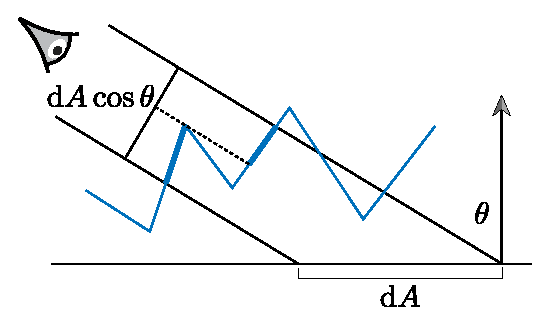
\includegraphics[width=0.5\linewidth]{Pictures/chap08/Microfacetvisiblearea.eps}
    \caption{从观察者或光源处看时,曲面上的微分面积变为$\mathrm{d}A\cos\theta$,
        其中$\cos\theta$是入射方向与曲面法线夹角的余弦。
        可见微面(粗线)的投影曲面面积也一定等于$\mathrm{d}A\cos\theta$;
        掩模遮挡函数$G_1$给出了$\mathrm{d}A$上的微面总面积中在给定方向可见的比例。}
    \label{fig:8.17}
\end{figure}

因为微面构成了高度场,所以每个背向微面遮住的正向微面面积
都等于它在方向$\bm\omega$的投影面积。
\refeq{8.12}中,如果$A^{+}({\bm\omega})$是从方向$\bm\omega$看到的
正向微面投影面积,而$A^{-}({\bm\omega})$是背向微面的投影面积,
则$\cos\theta=A^{+}({\bm\omega})-A^{-}({\bm\omega})$.
因此我们可以把掩模遮挡函数改写为可见微面面积与正向微面面积之比:
\begin{align*}
    G_1({\bm\omega})=\frac{A^{+}({\bm\omega})-A^{-}({\bm\omega})}{A^{+}({\bm\omega})}\, .
\end{align*}

掩模遮挡函数习惯上用一个辅助函数$\Lambda({\bm\omega})$来表示,
后者度量了单位可见微面面积内被遮挡不可见的微面面积。
\begin{align}
    \label{eq:8.13}
    \Lambda({\bm\omega})=\frac{A^{-}({\bm\omega})}{A^{+}({\bm\omega})-A^{-}({\bm\omega})}=\frac{A^{-}({\bm\omega})}{\cos\theta}\, .
\end{align}

方法\refvar[MicrofacetDistribution::Lambda]{Lambda}{()}计算该函数。对于每个微面分布它都有特定实现。
\begin{lstlisting}
`\refcode{MicrofacetDistribution Public Methods}{+=}\lastnext{MicrofacetDistributionPublicMethods}`
virtual `\refvar{Float}{}` `\initvar[MicrofacetDistribution::Lambda]{Lambda}{}`(const `\refvar{Vector3f}{}` &w) const = 0;
\end{lstlisting}

我们通过一些代数变换用$\Lambda({\bm\omega})$表示$G_1({\bm\omega})$:
\begin{align*}
    G_1({\bm\omega})=\frac{1}{1+\Lambda({\bm\omega})}\, ,
\end{align*}
因此我们利用\refvar[MicrofacetDistribution::Lambda]{Lambda}{()}来
提供方法\refvar[MicrofacetDistribution::G1]{G1}{()}。
\begin{lstlisting}
`\refcode{MicrofacetDistribution Public Methods}{+=}\lastnext{MicrofacetDistributionPublicMethods}`
`\refvar{Float}{}` `\initvar[MicrofacetDistribution::G1]{G1}{}`(const `\refvar{Vector3f}{}` &w) const {
    return 1 / (1 + `\refvar[MicrofacetDistribution::Lambda]{Lambda}{}`(w));
}
\end{lstlisting}

只是微面分布还不能施加足够的条件以明确一个特定的$\Lambda({\bm\omega})$函数;
许多函数都能满足\refeq{8.12}中的约束。
例如,如果我们假设微面上邻近点的高度之间没有关联,
则可能为给定的$D({\bm\omega}_{\mathrm{h}})$找到唯一的$\Lambda({\bm\omega})$
(对于许多微面模型来说都能找到解析解)。
尽管该基本假设在现实中不成立——对于实际的微面,
一点的高度通常接近邻近点的高度——但所得函数$\Lambda({\bm\omega})$与
从实际表面测量到的情况相比已经很精确了。

在邻近点高度无关的假设下,各向同性的Beckmann-Spizzichino分布的$\Lambda({\bm\omega})$是
\begin{align}
    \Lambda({\bm\omega})=\frac{1}{2}\left(\mathrm{erf}(a)-1+\frac{\mathrm{e}^{-a^2}}{a\sqrt{\pi}}\right)\, ,
\end{align}
其中$a=\displaystyle\frac{1}{\alpha\tan\theta}$,
而$\mathrm{erf}$是误差函数
\sidenote{译者注:为了减少理解障碍,这里笔者把函数$\mathrm{erf}$的
自变量改回成了$\Lambda({\bm\omega})$中所用的$a$.},
$\displaystyle\mathrm{erf}(a)=\frac{2}{\sqrt{\pi}}\int_0^a\mathrm{e}^{-x^2}\mathrm{d}x$.
